%%%%%%%%%%%%%%%%%%%%%%%%%%%%%%%%%%%%%%%%%%%%%%%%%%%%%%%%%%%%%%%%%%%%%%%%%%%
%
% Template for a LaTex article in English.
%
%%%%%%%%%%%%%%%%%%%%%%%%%%%%%%%%%%%%%%%%%%%%%%%%%%%%%%%%%%%%%%%%%%%%%%%%%%%

\documentclass{article}

%\usepackage[latin1]{inputenc}

\usepackage[english]{babel}
% AMS packages:
\usepackage{amsmath, amsthm, amsfonts, graphicx, float, caption, subfigure}

% Theorems
%-----------------------------------------------------------------
\newtheorem{thm}{Theorem}[section]
\newtheorem{cor}[thm]{Corollary}
\newtheorem{lem}[thm]{Lemma}
\newtheorem{prop}[thm]{Proposition}
\theoremstyle{definition}
\newtheorem{defn}[thm]{Definition}
\theoremstyle{remark}
\newtheorem{rem}[thm]{Remark}

% Shortcuts.
% One can define new commands to shorten frequently used
% constructions. As an example, this defines the R and Z used
% for the real and integer numbers.
%-----------------------------------------------------------------
\def\RR{\mathbb{R}}
\def\ZZ{\mathbb{Z}}

% Similarly, one can define commands that take arguments. In this
% example we define a command for the absolute value.
% -----------------------------------------------------------------
\newcommand{\abs}[1]{\left\vert#1\right\vert}

% Operators
% New operators must defined as such to have them typeset
% correctly. As an example we define the Jacobian:
% -----------------------------------------------------------------
\DeclareMathOperator{\Jac}{Jac}

%---------------------------------------------------------------

 
\begin{document}

\section*{Models}

We propose several models which include differents rotational velocities and optical depths. We also take into account the dust within the gas and two differents initial distributions of the photons, central and homogeneous. At the end we study 48 models, those are resumed in Table[1]\\
\\
\begin{table}[H]
\begin{center}
\begin{tabular}{|c|c|}
\hline
Velocity(km/s) & 50, 100, 200, 300\\
\hline
Optical Depth & $\tau = 10^{5},10^{6},10^{7}$\\
\hline
Photons Distributions & Central, Homogeneous\\
\hline
\end{tabular}
\caption{Models, If we take into account all these possibles combinations we get 24 models with dust and 24 without dust for a total of 48 models.}
\end{center}
\end{table}

We later study this models taking into account the posititon of the observer respect to the axis of rotation of the cloud.

\subsection*{Rotational Effect}

Due to the resonant nature of the lyman alpha line, gas kinematics play an important role in the shape of this line. In particular we study the case in which this gas is spherically symmetric and its rotating.\\

In cartesian coordinates the rotational velocity around de the z-axys is defined by:\\

\begin{subequations}
\begin{align}
    v_{x}=-\dfrac{y}{R}v \label{subeq1}\\
    v_{y}=\dfrac{x}{R}v \label{subeq2}
\end{align}
\end{subequations}
\\
Where $x$ and $y$ define de position of the gas atoms and dust particles. The minus sign in the x-component of the velocity is due to the direction of rotation, in this case we assume that as seeing from the top,the rotation is anticlockwise.\\   

In Figure[1] the effect that rotation have in the spectra is shown, for both distributions central (Left) and homogeneous (right). This is a general case in the sense that is independent of the position of an external observer. 

\begin{figure}[H]

  \centering

  \label{HOMandCentral}\caption{Shape of the lyman alpha line for differents velocities. The left panel show the central distribution while the right panel show the homogeneous distribution. }

  \begin{tabular}{cc}

    
    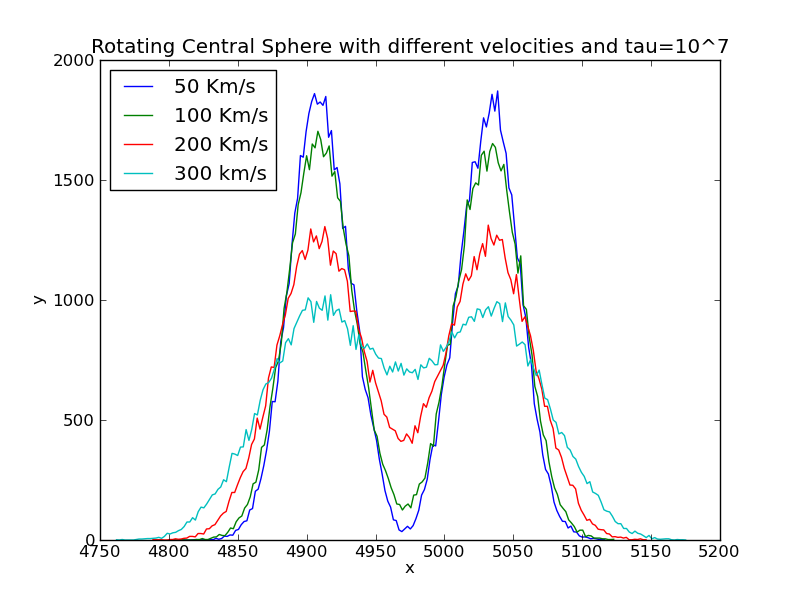
\includegraphics[width=60mm]{7tDifSpeedsZ.png}&

    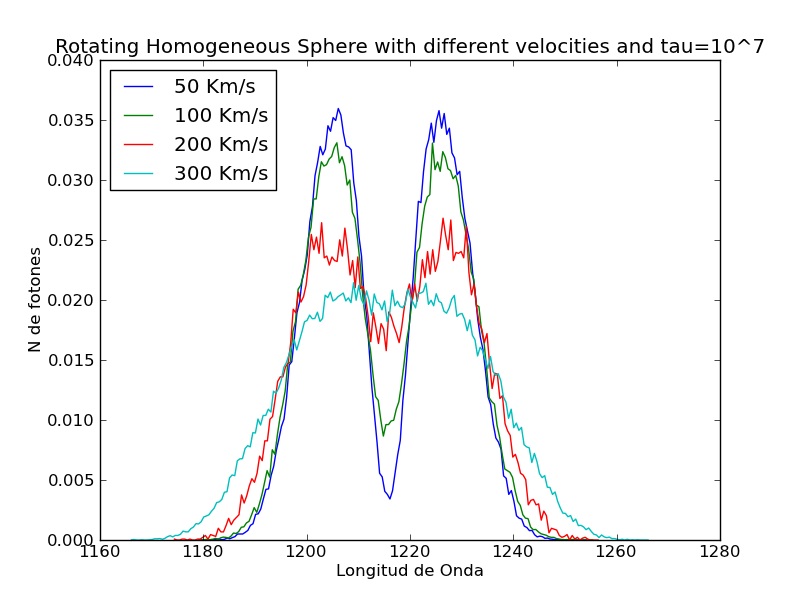
\includegraphics[width=60mm]{7tHOMDifSpeeds1.png}\\


  \end{tabular}

\end{figure}
Now if we take into account the position of the observer and compute this for differents angles of observation $\theta$ the outcoming spectra is modified as is shown in figure[2]. The main feature here is that as the angle increases the line high decreases. It means that a observer in the poles will observe a higher double peak than a observer in the ecuator. We will understand this in more details when we present the resaults of the scape fraction in section[].     

\begin{figure}[H]
\begin{center}
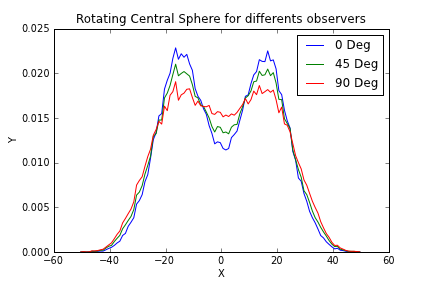
\includegraphics[scale=0.45]{Observers.png}
\end{center}
\caption{Spectra for different observers. Model:$V=300km/s$, Optical Depth $\tau=10^{7}$ and Central Distribution without dust.}
\end{figure}

%describir los modelos, poner las ecuaciones de la velocidad de rotacion, %poner las graficas para un modelo dado poner el efecto de la rotación (poner %uno con velocidad cero) y del observador.



\section*{Resaults and Discussion}
\label{sec:Results_ly_Rotation}

%Ver correo de Jaime y tratar de explicar a que se deben estos efectos.

In the previous section we describe the models that we study the effect of rotation in the Lyman alpha line and see the effect of rotation in the specrtums. Now we show the main resaults that we obtain, in particual we pay spetial attention to the position of the maximums, the width of the line and the escape fraction in function of the rotational velocity and the angle of observation $\theta$. 

\subsection*{Maximums Position}

\begin{figure}[H]

  \centering

  \label{figur}\caption{Width of the lyman-alpha line for all the models. }

  \begin{tabular}{cc}

    
    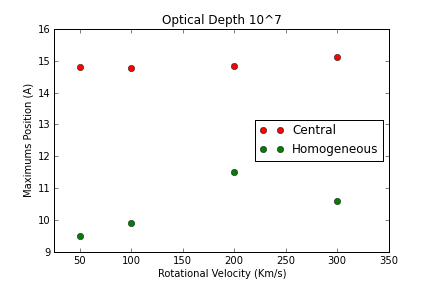
\includegraphics[width=40mm]{0maximum7t.png}&

    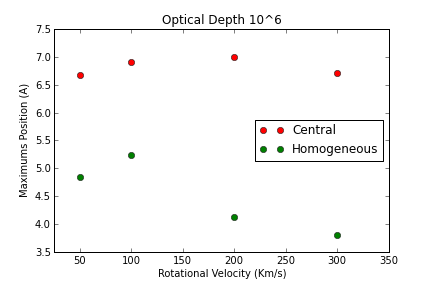
\includegraphics[width=40mm]{0maximum6t.png}

    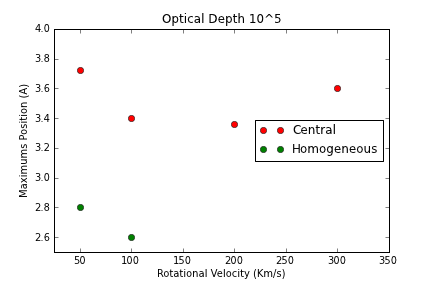
\includegraphics[width=40mm]{0maximum5t.png}

   \end{tabular}

\end{figure}
(comparar con la grafica del apendice de clara con el eje x el optical depth y en el eje-y los maximos)

The maximus position gives information about the wave lenght of the mayority of the outcoming photons after they interact with the gas, in addition as a photon have more scatterings its wave lenght would be larger than the initial which is $1216$ {\AA}.
As we can see in Fig.[3] the position of the maximums does not change with rotational velocity. But it change from homogeneous and central. 

\subsection*{Line Width}

%el ancho sirve para saber el rango de scattering que tienen los fotones.
Another effect that the rotation of the gas produce is in the  width of the lyman alpha line. The width of the line provide information of the the how many phtons scape with a particular wave lenght, in the ideal case in which all the photons scape with the same wave lenght the outcoming spectrum would be narrow. For all the models we study we found that as the rotational velocity increase as the line width increase this is show in Fig.[4].\\
 

\begin{figure}[H]

  \centering

  \label{figur}\caption{Width of the lyman-alpha line for all the models. }

  \begin{tabular}{cc}

    
    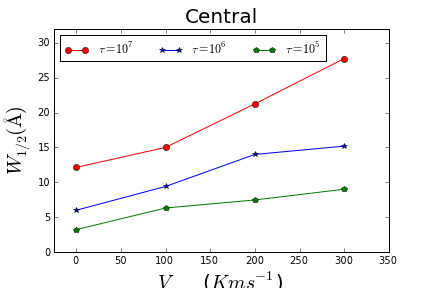
\includegraphics[width=60mm]{WidthCentral.png}&

    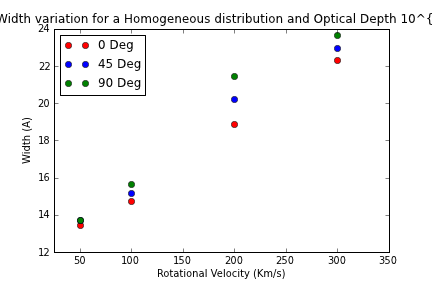
\includegraphics[width=60mm]{WidthHomogeneous.png}\\

    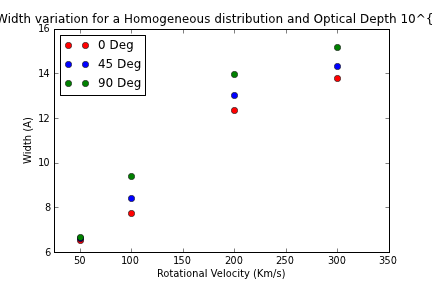
\includegraphics[width=60mm]{Width6.png}&

    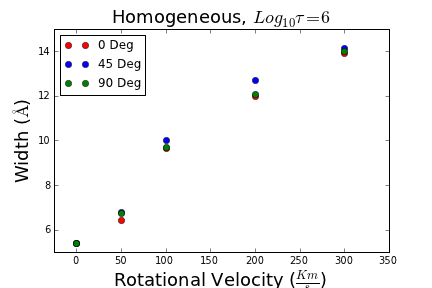
\includegraphics[width=60mm]{Width6HOM.png}\\

    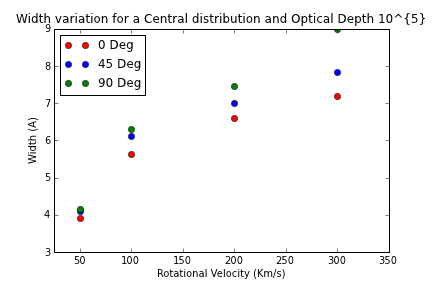
\includegraphics[width=60mm]{Width5.png}&

    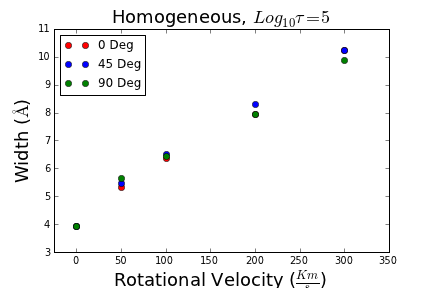
\includegraphics[width=60mm]{Width5HOM.png}\\

  \end{tabular}

\end{figure}

We also found that the width for a particular model is not the same for differents angles of observation in particular as the angle increase the width also increase, it means that as the angle increase the number of scatterings of the photons increasse for this reason we see a broader line. Fig.[5]\\

\begin{figure}[H]
\begin{center}
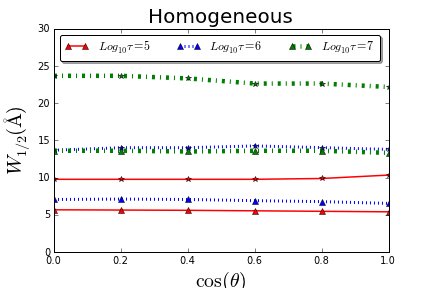
\includegraphics[scale=0.45]{WidthvsTheta.png}
\caption{Width variation in function of theta}
\end{center}
\end{figure}




\subsection*{Escape Fraction}

The fraction of photons that escape from de cloud of gas and dust is defined as:\\

\begin{equation}
F_{e}=\dfrac{\Sigma_{NI} \vec{k}\cdot \vec{o}}{\Sigma_{NF}\vec{k}\cdot \vec{o}}
\end{equation}

Where NI is the initial number of photons and NF is the final. This escape fraction is computed for all the models which resaults are shown in Fig.[6]\\
 
\begin{figure}[H]

  \centering

  \label{figur}\caption{Escape fraction for all the models. Left panels show the central distribution, while right panels show the homogeneous distribution}

  \begin{tabular}{cc}

    
    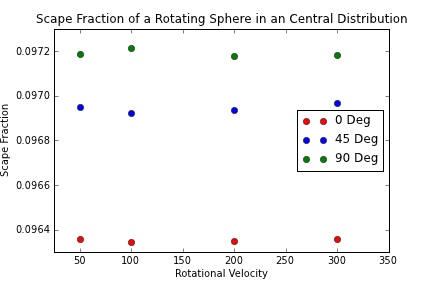
\includegraphics[width=60mm]{FECentral5.png}&

    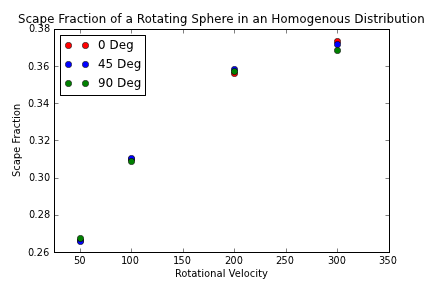
\includegraphics[width=60mm]{FEHOM5.png}\\

    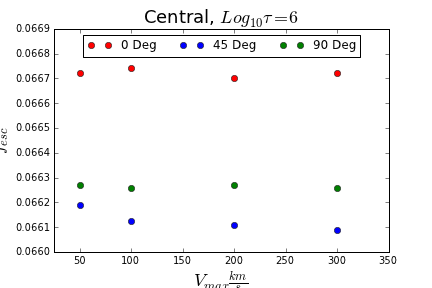
\includegraphics[width=60mm]{FECentral6.png}&

    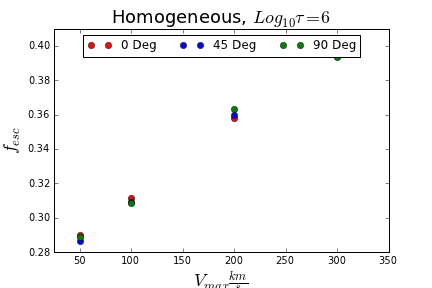
\includegraphics[width=60mm]{FEHOM6.png}\\

    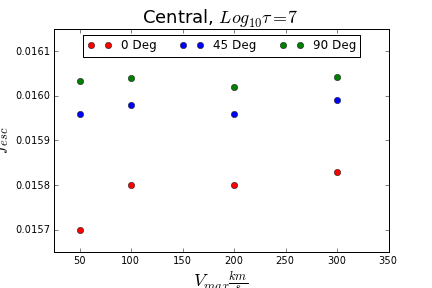
\includegraphics[width=60mm]{FECentral7.png}&

    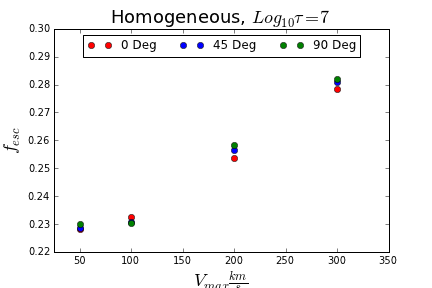
\includegraphics[width=60mm]{FEHOM7.png}\\

  \end{tabular}

\end{figure}

When the distribution is homogeneous the effect of velocity in the escape fraction is clear while in the central model the effect is not noterous.
The main effect is that the escape fraction increase as the velocity increase. 

\section*{Observational effect.}


\section*{Tables}

Maximos\\

\begin{table}[H]
\begin{center}
\begin{tabular}{|c|c|c|}
\hline          
Velocity (Km/s) & Maximum 1 position & Maximum 2 position \\ 
\hline 
50 & -16.2695 & 16.23705 \\ 
\hline 
100 & -15.66496 & 15.33504 \\ 
\hline 
200 & -16.93149 & 14.56851 \\ 
\hline 
300 & -13.40048 & 16.09952 \\ 
\hline 
\end{tabular} 
\caption{Optical Depth $\tau= 10^{7}$, Central Distribution}
\end{center}
\end{table}

\begin{table}[H]
\begin{center}
\begin{tabular}{|c|c|c|}
\hline 
Velocity (Km/s) & Maximum 1 position & Maximum 2 position\\ 
\hline 
50 & -7.46286 & 6.53714 \\ 
\hline 
100 & -7.53357 & 6.96643 \\ 
\hline 
200 & -8.17453 & 7.32547 \\ 
\hline 
300 & -6.81487 & 6.18513 \\ 
\hline 
\end{tabular} 
\end{center}
\caption{Optical Depth $\tau = 10^{6}$, Central Distribution}
\end{table}

\begin{table}[H]
\begin{center}
\begin{tabular}{|c|c|c|}
\hline 
Velocity(Km/s) & Maximum 1 position & Maximum 2 position\\ 
\hline 
50 & -4.33708 & 3.66292 \\ 
\hline 
100 & -4.27326 & 3.72674 \\ 
\hline 
200 & -3.7737 & 3.7263   \\ 
\hline 
300 & -3.84903 & 4.15097 \\ 
\hline 
\end{tabular}
\caption{Optical Depth $\tau=10^{5}$, Central distribution} 
\end{center}
\end{table}

Line width\\

\begin{table}[H]
\begin{center}
\begin{tabular}{|c|c|c|}
\hline 
Velocity(Km/s) & FWHM & $\theta$\\ 
\hline 
50 & 12.62 & $0^{o}$ \\ 
\hline 
50 & 12.72 & $45^{o}$ \\ 
\hline 
50 & 12.93 & $90^{o}$ \\ 
\hline 
100 & 14.07 & $0^{o}$ \\ 
\hline
100 & 14.48 & $45^{o}$ \\ 
\hline 
100 & 15.00 & $90^{o}$ \\ 
\hline 
200 & 16.90 & $0^{o}$  \\ 
\hline 
200 & 18.51 & $45^{o}$ \\ 
\hline 
200 & 21.24 & $90^{o}$ \\ 
\hline 
300 & $24.69^{*}$ & $0^{o}$ \\ 
\hline 
300 & $25.79^{*}$ & $45^{o}$  \\ 
\hline  
300 & $27.73^{*}$ & $90^{o}$ \\ 
\hline  
\end{tabular}
\caption{Lines Widhts for a Central Distribution and $\tau=10^{7}$} 
\end{center}
\end{table}


Scape fracton\\

\begin{table}[H]
\begin{center}
\begin{tabular}{|c|c|c|c|c|}
\hline 
Model & Velocity (km/s) & $\theta$ & Dust $\sum (s)$& $\sum (s)$\\ 
\hline 
Homogeneous & 50 & $0^{o}$& 13293.06 &49939.53\\ 
\hline 
Homogeneous & 50 & $45^{o}$& 13291.04 &50001.59\\ 
\hline 
Homogeneous & 50 & $90^{o}$ & 13348.76 &49922.73\\ 
\hline 
Homogeneous & 100 & $0^{o}$ & 15527.69 &50114.11\\ 
\hline
Homogeneous & 100 & $45^{o}$ & 15511.56 &49967.17\\ 
\hline
Homogeneous & 100 & $90^{o}$ & 15401.71 & 49833.65\\ 
\hline 
Homogeneous & 200 & $0^{o}$  & 17830.85 & 50078.69\\ 
\hline 
Homogeneous & 200 & $45^{o}$ & 17932.87 & 50064.42\\ 
\hline 
Homogeneous & 200 & $90^{o}$ & 17830.85  & 49931.748\\ 
\hline
Homogeneous & 300 & $ 0^{o}$ & 18687.33 & 50048.33 \\ 
\hline 
Homogeneous & 300 & $45^{o}$ & 18572.12& 49922.67\\ 
\hline  
Homogeneous & 300 & $90^{o}$ & 18421.79 & 49979.37\\ 
\hline  
\end{tabular}
\caption{Escape fraction for a Homogeneous Distribution and optical depth $10^{5}$.} 
\end{center}
\end{table}


\begin{table}[H]
\begin{center}
\begin{tabular}{|c|c|c|c|c|}
\hline 
Model & Velocity (km/s) & $\theta$ & Dust $\sum (s)$& $\sum (s)$ \\ 
\hline 
Central & 50 & $0^{o}$ & 4809.881 & 49917.069 \\ 
\hline 
Central & 50 & $45^{o}$ & 4829.21 & 49811.79 \\ 
\hline 
Central & 50 & $90^{o}$ & 4845.108 & 49853.039\\ 
\hline 
Central & 100 & $0^{o}$ & 4809.665 & 49921.30 \\  
\hline
Central & 100 & $45^{o}$ & 4828.65 & 49820.13 \\ 
\hline
Central & 100 & $90^{o}$ & 4846.45 & 49854.0 \\ 
\hline 
Central & 200 & $0^{o}$  & 4809.63 & 49917.64 \\ 
\hline 
Central & 200 & $45^{o}$ & 4829.25 & 49818.49 \\ 
\hline 
Central & 200 & $90^{o}$ & 4844.89 & 49856.66 \\ 
\hline 
Central & 300 & $ 0^{o}$ & 4810.56 & 49922.98\\ 
\hline 
Central & 300 & $45^{o}$ & 4831.16 & 49823.33\\ 
\hline  
Central & 300 & $90^{o}$ & 4845.33 & 49858.48\\ 
\hline  
\end{tabular}
\caption{Escape fraction for the central Distribution and optical depth $10^{5}$.} 
\end{center}
\end{table}


% Bibliography
%-----------------------------------------------------------------
%\begin{thebibliography}{99}

%\bibitem{Cd94} Author, \emph{Title}, Journal/Editor, (year)

%\end{thebibliography}

\end{document}
